\documentclass[
	aspectratio=169, % default is 43
	8pt, % font size, default is 11pt
	handout, % handout mode without animations, comment out to add animations
]{beamer}

\documentclass[
	aspectratio=169, % default is 43
	8pt, % font size, default is 11pt
	handout, % handout mode without animations, comment out to add animations
]{beamer}

\usepackage{../template/beamerthemeuulm} % use the inofficial uulm beamer theme
\setfaculty{infIngPsy} % set the color scheme for your faculty here [med/infIngPsy/math/nat]

% requires symbolic links
% git clone git@github.com:SoftVarE-Group/SlideTemplate.git C:\Users\...\SlideTemplate
% mklink /J template C:\Users\...\SlideTemplate
% git clone git@spgit.informatik.uni-ulm.de:thuem/slides.git C:\Users\...\ThomasSlides
% mklink /J thomasslides C:\Users\...\ThomasSlides
\graphicspath{{../template/pics/logos}{../template/pics/nature}{../template/pics/uulm}{../thomasslides/}{../pics/people/}{../pics/xkcd/}}

%\usepackage[ngerman]{babel} % use this line for slides in German
%\recordingtrue % special recording mode for use with a greenscreen, gives you space to show yourself in a layer in front of the slides, has no effect in the handout mode

\title{Software Product Lines} % short title is used for the slide footer but optional

% LINKED LITERATURE

\newcommand{\ludewiglichter}{\href{https://learning.oreilly.com/library/view/-/9781457184932/?ar}{Ludewig and Lichter}}
\newcommand{\seeconomics}{\href{https://rds-ulm.ibs-bw.de/link?kid=027381854}{SE Economics}}
\newcommand{\sommervillelink}[1]{\href{https://ulm.ibs-bw.de/aDISWeb/app?service=direct/0/Home/$DirectLink\&sp=SOPAC00\&sp=SAKSWB-IdNr1615420983}{#1}}
\newcommand{\sommerville}{\sommervillelink{Sommerville}}
\newcommand{\thehumbleprogrammer}{\href{https://dl.acm.org/doi/10.1145/1283920.1283927}{The Humble Programmer}}
\newcommand{\thepragmaticprogrammer}{\href{https://learning.oreilly.com/library/view/the-pragmatic-programmer/9780135956977/}{The Pragmatic Programmer}}

% TYPICAL COMMANDS FOR LECTURES

\renewcommand{\emph}[1]{{\color{blue}\textbf{#1}}}

\newcommand{\deutsch}[1]{{\color{blue}(#1)}}
\newcommand{\deutschertitel}[1]{{\tiny\deutsch{#1}}}

\newcommand{\mycite}[1]{``#1''}
\newcommand{\mytitlesource}[1]{{\tiny\normalfont\mbox{[#1]}}}
\newcommand{\mysource}[1]{\ifthenelse{\equal{#1}{}}{}{\phantom{.}~\hfill~\mytitlesource{#1}}}

\newcommand{\todo}[1]{{\color{red}\textbf{[#1]}}}
\newcommand{\fodo}[1]{\todo{\footnote{\todo{#1}}}}
\newcommand{\todots}{\todo{\ldots}}

% IMPORTED PACKAGES

%\usepackage{adjustbox} % used for partofpage
%\usepackage{tcolorbox} % used for mydefinition, mynote, myexample
\usepackage{multicol} % used temporarily for the lecture overview
\usepackage{mathtools} % required for absolute value in modeling lecture

% COMMANDS TO LAYOUT AND ANNIMATE SLIDES

\newcommand{\lessonslearned}[3]{
	\subsection{Summary}
	\begin{frame}{\insertsection -- \insertsubsection}
		\leftorright{
			\mydefinition{Lessons Learned}{
				\begin{itemize}
					#1
				\end{itemize}
			}
			\mynote{Further Reading}{
				\small % references take space, can be a little smaller
				\begin{itemize}
					#2
				\end{itemize}
			}
		}{
			\myexample{Practice}{
				#3
			}
		}
	\end{frame}
}

% TODO temporary hack to layout the slide overview in two colums
\renewcommand{\lectureoverview}{
%	\section*{Overview}
%	\subsection*{Overview}
	\begin{frame}{\insertsubtitle}
		\begin{multicols}{2}
			\tableofcontents
		\end{multicols}
	\end{frame}
}

\renewcommandx{\maketitle}[2][1=apr21-o25a,2=150]{
    {
	\usebackgroundtemplate{} % TODO temporary hack to enable missing pictures at title slide
	%\ifx {#1} \empty \else {\usebackgroundtemplate{\includegraphics[trim=0 0 0 #2,clip,width=\paperwidth]{#1}}} \fi     
	%\usebackgroundtemplate{\includegraphics[trim=0 0 0 #2,clip,width=\paperwidth]{#1}}
    \begin{frame}[plain]
        \vskip0pt plus 1filll
        \begin{beamercolorbox}[wd=\paperwidth,ht=4.5ex,dp=2ex,right]{titlebox}
            \LARGE\textbf{\inserttitle}\hspace*{20pt}
        \end{beamercolorbox}%
        \nointerlineskip%
        \begin{beamercolorbox}[wd=\paperwidth,ht=2.25ex,dp=1ex,right]{subtitlebox}
            \small 
            \ifx \insertsubtitle \empty \else \insertsubtitle\ $\vert$ \fi
            \insertauthor\
            \ifx \insertdate \empty \else $\vert$ \insertdate \fi
            \hspace*{20pt}
        \end{beamercolorbox}%
        \nointerlineskip%
        \begin{beamercolorbox}[wd=\paperwidth,ht=4.5ex,dp=2ex,left]{logobox}
            \centering
            \vspace{-1ex}
            \hspace{10pt}
            \includegraphics[height=4.5ex]{sp} % SPECIFY INSTITUTE LOGO HERE
            \hfill
            \includegraphics[height=4.5ex]{uulm}
            \hspace{10pt}
        \end{beamercolorbox}%
    \end{frame}
    }  
}

%
%\newcommand{\onlyleft}[1]{
%	\halfpage{#1}
%}
%
%\newcommand{\onlyright}[1]{
%	~\hfill
%	\halfpage{#1}
%}
%
%\newcommand{\leftorright}[2]{
%	\uncover<1>{\halfpage{#1}}
%	\hfill
%	\uncover<3->{\halfpage{#2}}
%}
%
%\newcommand{\rightorleft}[2]{
%	\uncover<3->{\halfpage{#1}}
%	\hfill
%	\uncover<1>{\halfpage{#2}}
%}
%
%\newcommand{\leftthenright}[2]{
%	\halfpage{#1}
%	\hfill\pause
%	\halfpage{#2}
%}
%
%\newcommand{\leftandright}[2]{
%	\halfpage{#1}
%	\hfill
%	\halfpage{#2}
%}
%
%\newcommand{\leftmiddleandright}[3]{
%	\thirdpage{#1}
%	\hfill
%	\thirdpage{#2}
%	\hfill
%	\thirdpage{#3}
%}
%
%\newcommand{\leftmiddleorright}[3]{
%	\uncover<1>{\thirdpage{#1}}
%	\hfill
%	\uncover<3>{\thirdpage{#2}}
%	\hfill
%	\uncover<5->{\thirdpage{#3}}
%}
%
%\newcommand{\halfpage}[1]{\partofpage{48}{#1}}
%
%\newcommand{\thirdpage}[1]{\partofpage{31}{#1}}
%
%\newcommand{\partofpage}[2]{
%	\adjustbox{valign=t}{\begin{minipage}{0.#1\textwidth}
%			\begin{flushleft}
%				#2
%			\end{flushleft}
%	\end{minipage}}
%}
%
%\newcommand{\mydefinition}[2]{
%	\begin{tcolorbox}[title=#1,colback=orange!10,colframe=orange!30,coltitle=black,fonttitle=\bfseries,left=1mm,right=1mm,top=1mm,bottom=1mm]
%		\begin{flushleft}
%			#2
%		\end{flushleft}
%	\end{tcolorbox}
%}
%
%\newcommand{\mydefinitiontight}[2]{
%	\begin{tcolorbox}[title=#1,colback=white,colframe=orange!30,coltitle=black,fonttitle=\bfseries,left=0mm,right=0mm,top=0mm,bottom=0mm]
%		\begin{flushleft}
%			#2
%		\end{flushleft}
%	\end{tcolorbox}
%}
%
%\newcommand{\mynote}[2]{
%	\begin{tcolorbox}[title=#1,colback=red!10,colframe=red!30,coltitle=black,fonttitle=\bfseries,left=1mm,right=1mm,top=1mm,bottom=1mm]
%		\begin{flushleft}
%			#2
%		\end{flushleft}
%	\end{tcolorbox}
%}
%
%\newcommand{\myexample}[2]{
%	\begin{tcolorbox}[title=#1,colback=blue!10,colframe=blue!30,coltitle=black,fonttitle=\bfseries,left=1mm,right=1mm,top=1mm,bottom=1mm]
%		\begin{flushleft}
%			#2
%		\end{flushleft}
%	\end{tcolorbox}
%}
%
%\newcommand{\myexampletight}[2]{
%	\begin{tcolorbox}[title=#1,colback=white,colframe=blue!30,coltitle=black,fonttitle=\bfseries,left=0mm,right=0mm,top=0mm,bottom=0mm]
%		\begin{flushleft}
%			#2
%		\end{flushleft}
%	\end{tcolorbox}
%}


% Code Listings
\usepackage{listings}

\lstset{ 
	language=Java, % choose the language of the code
	numbers=none, % where to put the line-numbers
	numberstyle=\tiny, % the size of the fonts that are used for the line-numbers     
	showspaces=false, % show spaces adding particular underscores
	showstringspaces=false, % underline spaces within strings
	showtabs=false, % show tabs within strings adding particular underscores
	frame=single, % adds a frame around the code
	framerule=1pt,
	framesep=3pt,
	tabsize=2, % sets default tabsize to 2 spaces
	rulesepcolor=\color{gray},
	rulecolor=\color{black},
	captionpos=b, % sets the caption-position to bottom
	breaklines=true, % sets automatic line breaking
	breakatwhitespace=false, 
	moredelim=**[is][\color{red}]{@}{@},
	moredelim=**[is][\color{green}]{?}{?},
	moredelim=**[is][\color{blue}]{~}{~},
	escapeinside={(*@}{@*)},
	columns=fullflexible, 
	backgroundcolor=\color{white}
}

% Tables
\usepackage{booktabs}

\subtitle{2. Runtime Variability and Design Patterns}
\author{Timo Kehrer}

\begin{document}

\mode<handout>{\contentoverview}

\mode<beamer>{
	\ifdefined\thepicture
		\maketitle[\thepicture][\thepictureoffset]
	\else
		\maketitle[]
	\fi
}

% shared slide content

% introduced: 02a-configuration
% reused: 03a-intro
\newcommand{\frameImplementSPLs}{
	\begin{mycolumns}[widths={45},animation=none]
		\pic[width=\linewidth]{metaproduct2}
	\mynextcolumn
		\begin{note}{Key Issues}
			\begin{itemize}
			\item Systematic reuse of implementation artifacts
			\item Explicit handling of variability
			\end{itemize}
		\end{note}
		\uncover<2->{\begin{definition}{Variability\mysource{\fospl\mypage{48}}}
			\mycite{\emph{Variability} is the ability to derive different products from a common set of artifacts.}
		\end{definition}}
		~
		\uncover<3->{\begin{note}{Variability-Intensive System}
			Any software product line is a variability-intensive system. % TODO Timo: do we really need this term? where does this definition come from?
		\end{note}}
	\end{mycolumns}
}

% introduced: 02a-configuration
% reused: 02b-implementation, 03a-intro
\newcommand{\frameVariabilityAndBindingTimes}{
	\begin{mycolumns}[widths={55},animation=none]
		\begin{definition}{Binding Time \deutsch{Bindungszeitpunkt}\mysource{\fospl\mypage{48}}}
			\begin{itemize}
				\item Variability offers choices
				\item Derivation of a product requires to make decisions (aka. binding)
				\item Decisions may be bound at different binding times
			\end{itemize}
		\end{definition}
		~
		\uncover<2->{\begin{note}{When? By whom? How?}
			\lectureruntime\parta: \emph{when} and \emph{by whom}

			\lectureruntime\partb: \emph{how}
		\end{note}}
	\mynextcolumn
		\pic[width=\linewidth]{metaproduct2}
	\end{mycolumns}
}

% introduced: 03a-intro
% reused: 03a-intro
\newcommand{\frameRuntimeVariabilityProblems}{
	\begin{note}{Problems of Runtime Variability}
		{\bf Conditional Statements:}
		\begin{itemize}
			\item Code scattering, tangling, and replication
		\end{itemize}
		{\bf Design Patterns for Variability:}
		\begin{itemize}
			\item Trade-offs and potential negative side effects
			\item Constraints that may restrict their usage
		\end{itemize}
		{\bf In General:}
		\begin{itemize}
			\item Variable parts are always delivered
			\item Not well-suited for compile-time binding
		\end{itemize}
	\end{note}
}

% introduced: 03a-intro
% reused: 03a-intro
\newcommand{\frameSoftwareConfigurationManagement}{
	\begin{mycolumns}
		\begin{definition}{Software Configuration Management} % TODO source missing
			Policies, processes, and tools for managing evolving software systems:
			\begin{itemize}
				\item Version control
				\item System building
				\item Release management
				\item Change management
				\item Collaborative work
			\end{itemize}
		\end{definition}
	\mynextcolumn
		\begin{note}{No Software Configuration Management}
			\lecturecloneandown\parta: Ad-Hoc Clone-and-Own

			aka.\ unmanaged clone-and-own
		\end{note}
		\begin{note}{Version Control}
			\lecturecloneandown\partb: Clone-and-Own with Version Control

			instance of managed clone-and-own
		\end{note}
		\begin{note}{System Building}
			\lecturecloneandown\partc: Clone-and-Own with Build Systems

			instance of managed clone-and-own
		\end{note}
	\end{mycolumns}
}


% runtime variability
%   input: flags in source code, configuration files, runtime parameters (avoid recompilation)
%   realization: if, switch, encoded in objects/state, inheritance
%   design patterns for variability / OOP + outlook beyond runtime variability

\section{Configuration of Runtime Variability}

%\begin{frame}{Variants of Graphs and Their Features}
	%\centering
	%\includegraphics[width=.7\linewidth,page=6,trim=20 20 20 150,clip]{FeatureIDE with Graphs/2016-05-19 ICSE FeatureIDEdemo}
	%% TODO export into separate PDF containing only the separate products
%\end{frame}
%
%\subsection{Runtime Parameters}
%\begin{frame}{\insertsubsection}
	%\leftorright{
		%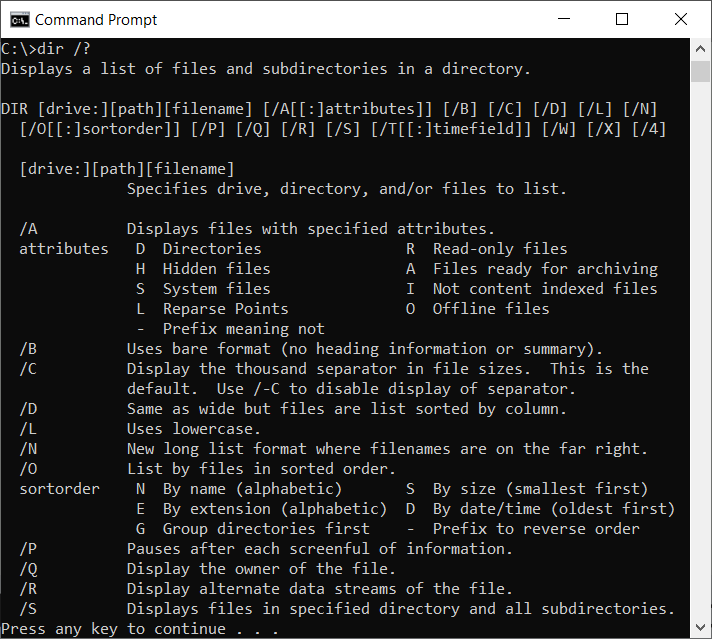
\includegraphics[width=\linewidth]{runtime-parameters-win10-cmd-dir}
	%}{
		%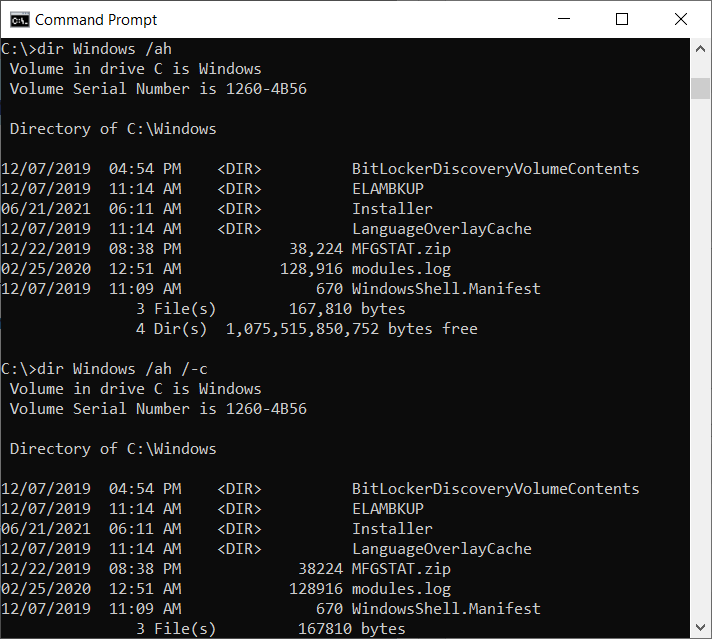
\includegraphics[width=\linewidth]{runtime-parameters-win10-cmd-dir2}
	%}
%\end{frame}

\subsection{Configuration Parameters}

\begin{frame}{Command-Line Options}
	\leftorright{
		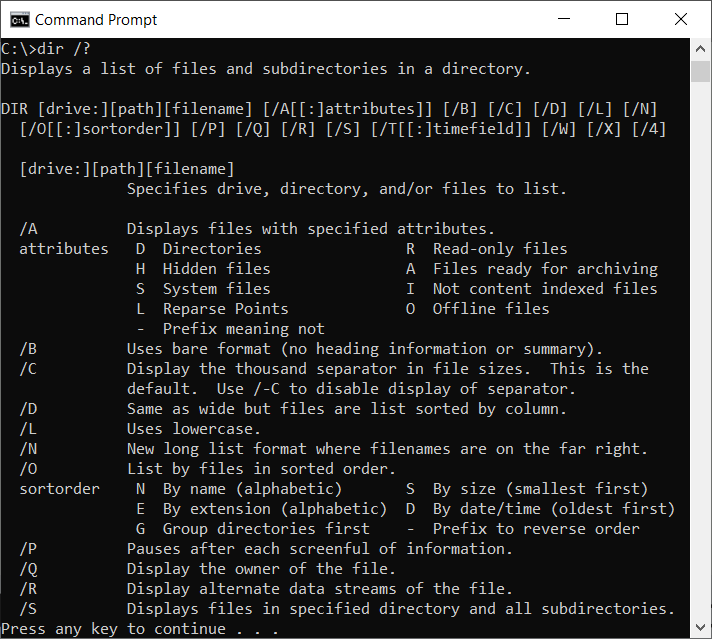
\includegraphics[width=\linewidth]{runtime-parameters-win10-cmd-dir}
	}{
		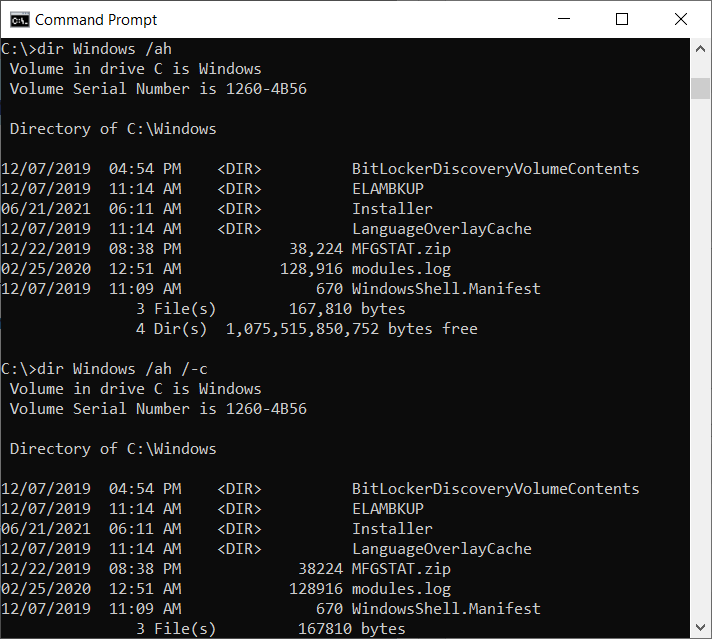
\includegraphics[width=\linewidth]{runtime-parameters-win10-cmd-dir2}
	}
\end{frame}

\begin{frame}{Configuration Files}
	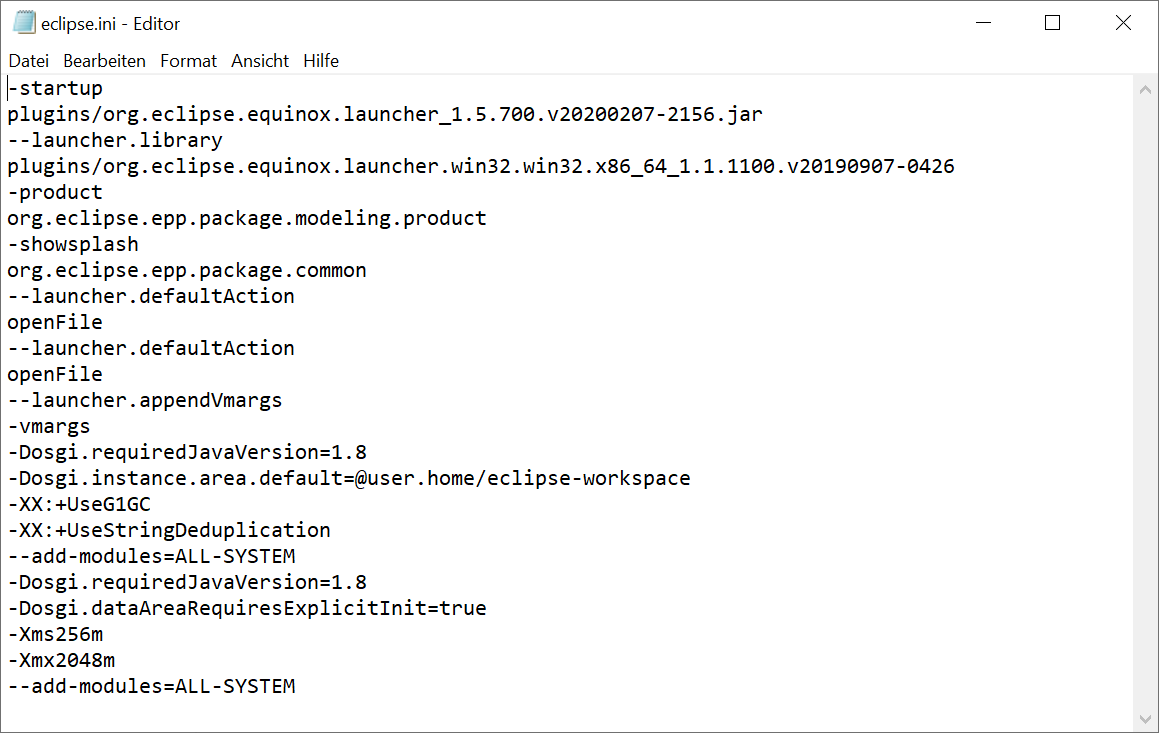
\includegraphics[width=0.75\linewidth]{configfile-eclipse-ini}
\end{frame}

\begin{frame}{Preference Dialogs}
	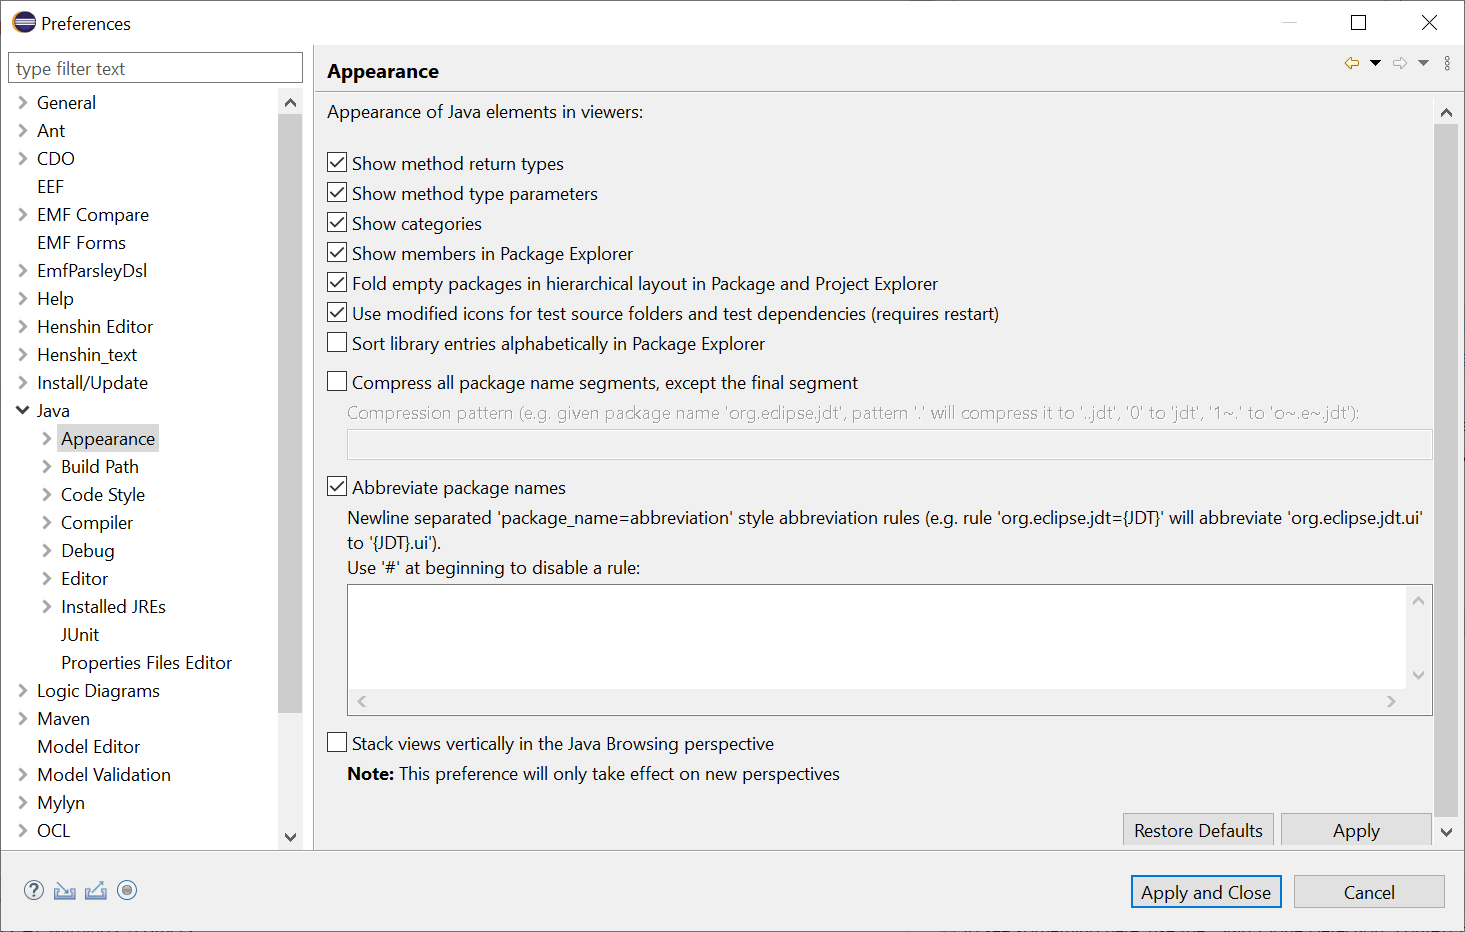
\includegraphics[width=0.75\linewidth]{preferences-eclipse}
\end{frame}

\begin{frame}{Common Principle: Configuration Parameters}
	\leftorright{
		\myexampletight{Command-Line Options}{
			\begin{center}
				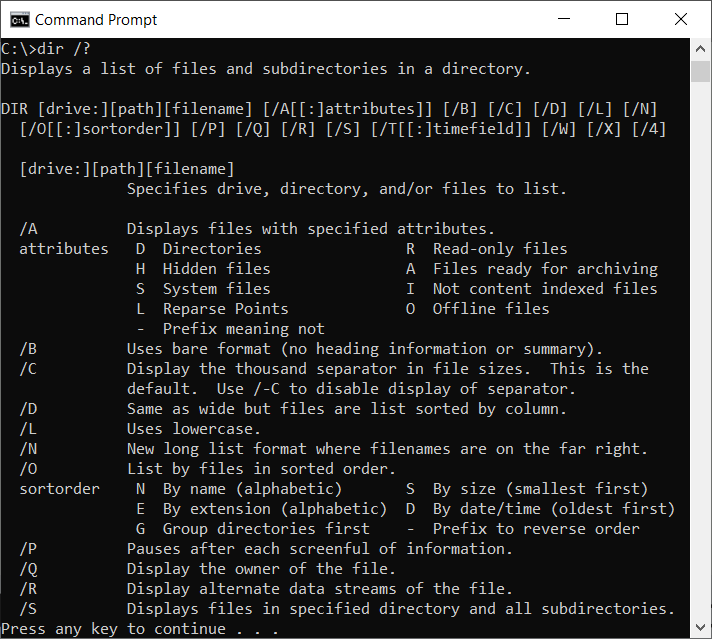
\includegraphics[width=0.7\linewidth,height=0.125\textheight]{runtime-parameters-win10-cmd-dir}
			\end{center}
		}
		\myexampletight{Configuration Files}{
			\begin{center}
				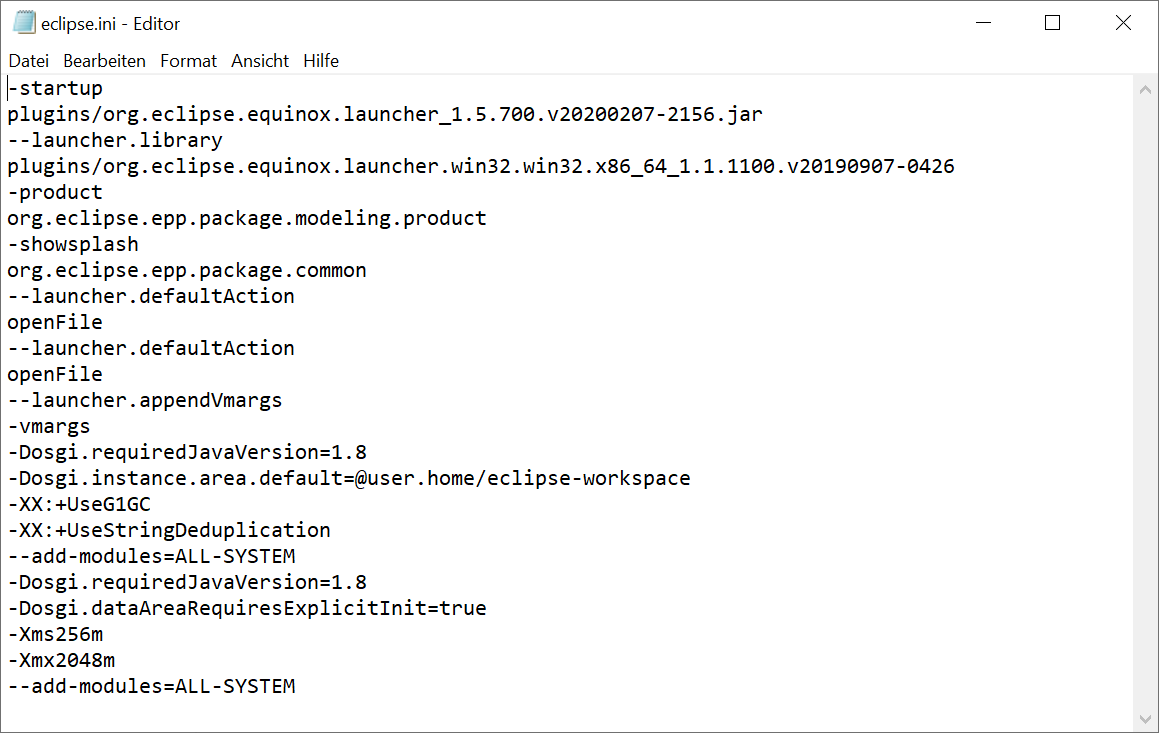
\includegraphics[width=0.7\linewidth,height=0.125\textheight]{configfile-eclipse-ini}
			\end{center}
		}
		\myexampletight{Preference Dialogs}{
			\begin{center}
				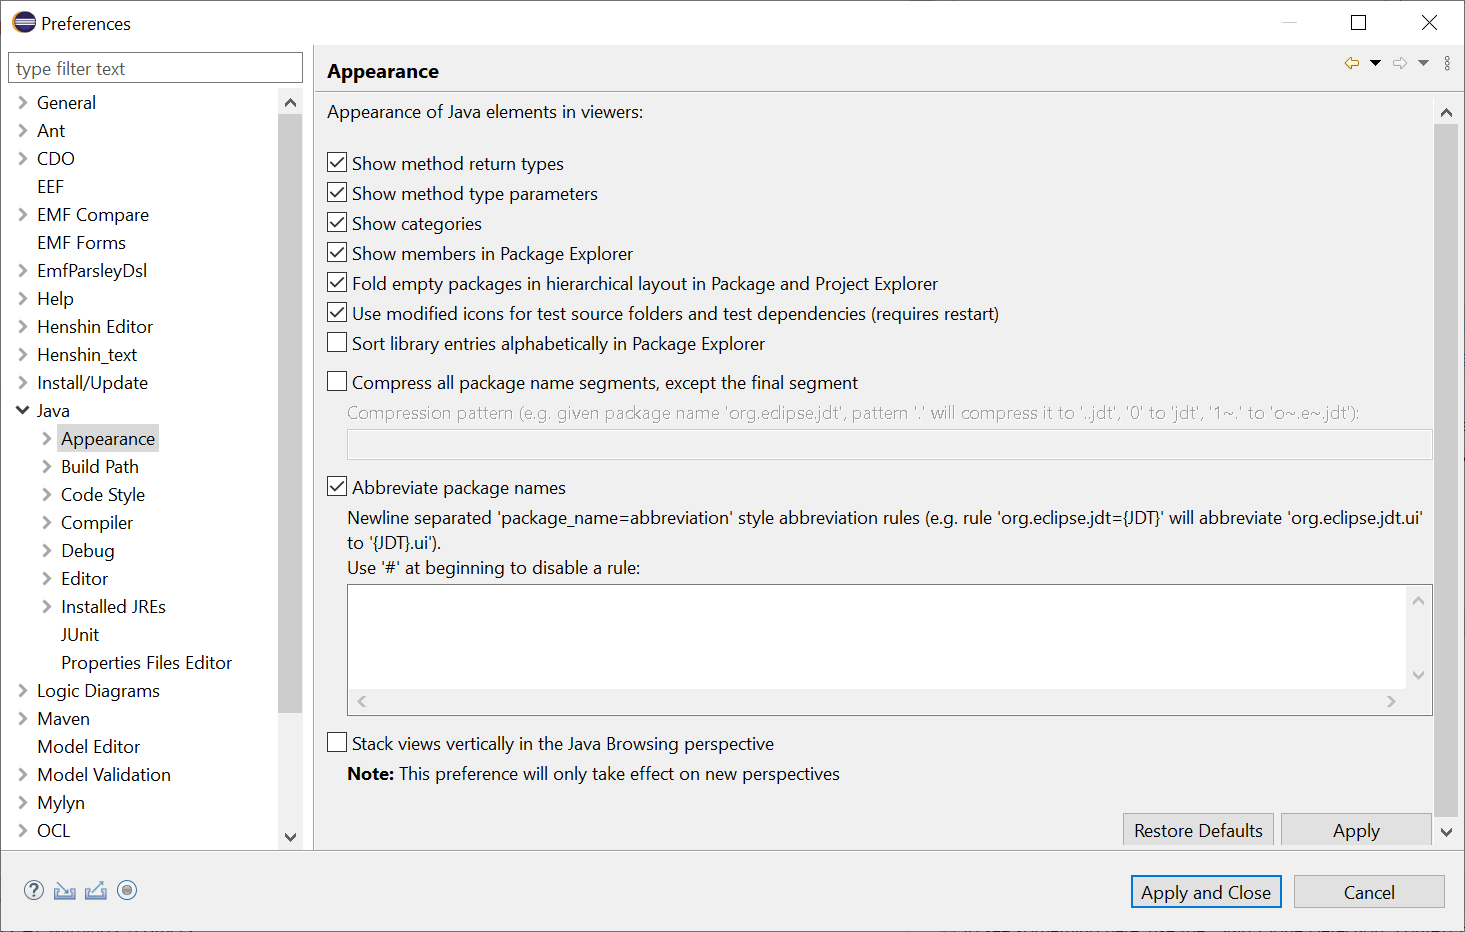
\includegraphics[width=0.7\linewidth,height=0.125\textheight]{preferences-eclipse}
			\end{center}
		}
	}{
		\mynote{Configuration Parameters}{
			\begin{itemize}
				\item Behavior of a program is determined by configuration parameters being interpreted at runtime.
				\item Configuration may happen non-interactively (at startup) or interactively (through dialogs).
			\end{itemize}
		}
	}
\end{frame}

\subsection{Example: A Graph Library}

\begin{frame}{\insertsubsection}
	A simple library providing \ldots \\
	\vspace{5mm}
	\leftorright{
		\myexample{\ldots graph data structures}{
			\begin{itemize}
				\item Directed/undirected edges
				\item Weighted/unweighted edges 
				\item Colored/uncolored nodes
				\item etc.
			\end{itemize}
		}		
	}{
		\myexample{\ldots and algorithms}{
			\begin{itemize}
				\item Vertex numbering
				\item Vertex coloring 
				\item Shortest path
				\item Minimum spanning tree 
				\item etc.
			\end{itemize}
		}
	}
\end{frame}

\subsection{Features as Configuration Parameters}
\begin{frame}{Features of a Graph as Configuration Parameters}
	\leftorright{
		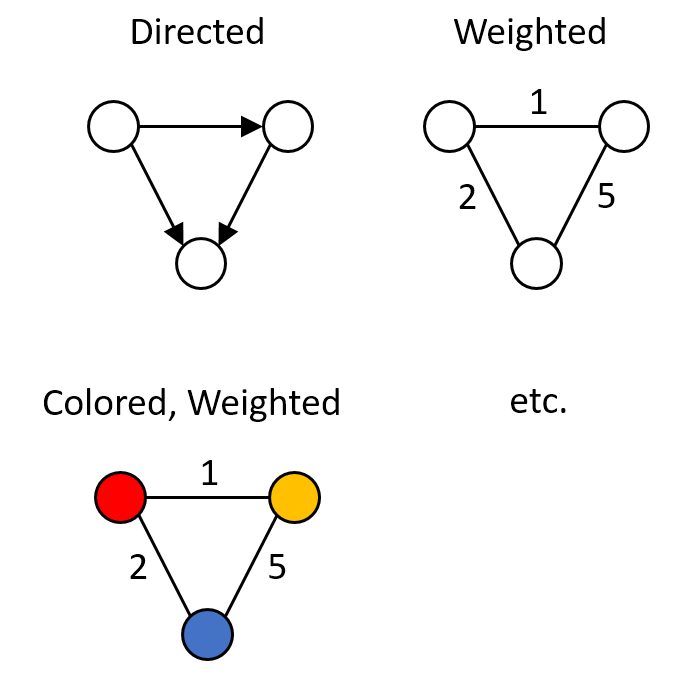
\includegraphics[width=0.9\linewidth]{graph-features}
	}{
		\mynote{}{
			\begin{itemize}
				\item Typically, configuration parameters are flags.
				\item Their boolean value determines which features are activated and which ones are deactivated.
			\end{itemize}
		}
	}
\end{frame}





\subsection{Validity of Parameter Settings}
\begin{frame}{\insertsubsection}
	\begin{columns}
		\column{.6\textwidth}
			\begin{tabular}{llll}
			\toprule
			{\bf Algorithm} 							& {\bf Graph type} 	& {\bf Weights} & {\bf Coloring}  \\ \midrule
			{\em Vertex numbering}			  & *          				& *        			& *         			\\
			{\em Vertex coloring}       	& undirected 				& *        			& colored   			\\
			{\em Shortest path}        		& directed   				& weighted 			& *         			\\
			{\em Minimum spanning tree} 	& undirected 				& weighted 			& *         			\\
			\ldots         					& \ldots 			 			& \ldots 		  	& \ldots 					\\ \bottomrule
			\end{tabular}
			\vspace{5mm}	
			\mynote{Dependencies between features must be checked}{
				\begin{itemize}
					\item When the parameters are configured at startup, or
					\item whenever parameters are changed at runtime.
				\end{itemize}
			}
		\column{.35\textwidth}
			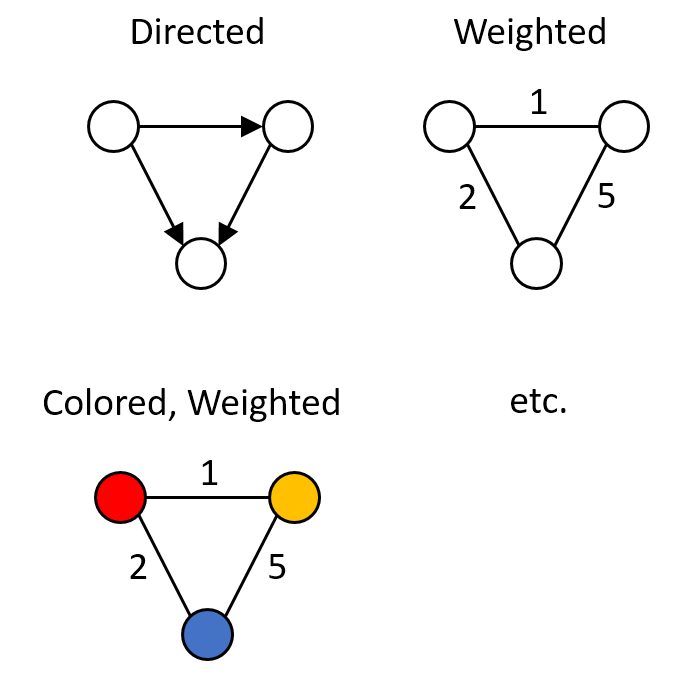
\includegraphics[width=\linewidth]{graph-features}
	\end{columns}
\end{frame}



\lessonslearned{
	\item External setting of configuration parameters through, e.g.,
		%\begin{itemize}
			command-line parameters,
			configuration files, or
			preference dialogs.
		%\end{itemize}
	\item Validity of parameter settings (i.e., feature combinations) may be affected by dependencies between features.
}{
	\item S. Apel, D. Batory, C. Kästner, and G. Saake. Feature-Oriented Software Product Lines - Concepts and Implementation. Springer, 2013. Chapter 4
	\item J. Meinicke, T. Thüm, R. Schröter, F. Benduhn, T. Leich, and G. Saake. Mastering Software Variability with FeatureIDE. Springer, 2017. Chapter 17.1
}{
	\item Do you know any practical examples making use of runtime variability?
	\item How does the configuration take place?
	\item Is the configuration checked for validity?
}

\sectionend
	
\section{Realization of Runtime Variability}

\subsection{A Non-Variable Graph Implementation}
\begin{frame}[fragile]{\insertsubsection}
	\begin{tiny}
		\begin{columns}
			\column{.45\textwidth}
\begin{lstlisting}
public class Graph {
	List nodes = new ArrayList();
	List edges = new ArrayList();

	Edge add(Node n, Node m) {
		Edge e = new Edge(n, m);
		nodes.add(n); nodes.add(m); edges.add(e);
		e.weight = new Weight();
		return e;
	}
	Edge add(Node n, Node m, Weight w) {
		Edge e = new Edge(n, m);
		nodes.add(n); nodes.add(m); edges.add(e);
		e.weight = w;
		return e;
	}
	void print() {
		for (int i = 0; i < edges.size(); i++) {
			((Edge) edges.get(i)).print();
		}
	}
}
\end{lstlisting}
\begin{lstlisting}
public class Color {
	static void setDisplayColor(Color c) {...}
}
\end{lstlisting}	
			\column{.45\textwidth}
\begin{lstlisting}
public class Node {
	int id = 0;
	Color color = new Color();

	void print() {
		Color.setDisplayColor(color);
		System.out.print(id);
	}
}
\end{lstlisting}
\begin{lstlisting}
public class Edge {
	Node a, b;
	Weight weight = new Weight();

	Edge(Node _a, Node _b) {
		a = _a; b = _b;
	}
	void print() {
		a.print(); b.print();
		weight.print();
	}
}
\end{lstlisting}
\begin{lstlisting}
public class Weight {
	void print() {...}
}
\end{lstlisting}
		\end{columns}
	\end{tiny}
\end{frame}

\begin{frame}[fragile]{``Symbolic'' Feature Traces}
	\begin{tiny}
		\begin{columns}
			\column{.45\textwidth}
\begin{lstlisting}
public class Graph {
	List nodes = new ArrayList();
	List edges = new ArrayList();

	Edge add(Node n, Node m) {
		Edge e = new Edge(n, m);
		nodes.add(n); nodes.add(m); edges.add(e);
		@e.weight = new Weight();@
		return e;
	}
	@Edge add(Node n, Node m, Weight w) {
		Edge e = new Edge(n, m);
		nodes.add(n); nodes.add(m); edges.add(e);
		e.weight = w;
		return e;
	}@
	void print() {
		for (int i = 0; i < edges.size(); i++) {
			((Edge) edges.get(i)).print();
		}
	}
}
\end{lstlisting}
\begin{lstlisting}
~public class Color {
	static void setDisplayColor(Color c) {...}
}~
\end{lstlisting}	
			\column{.45\textwidth}
\begin{lstlisting}
public class Node {
	int id = 0;
	~Color color = new Color();~

	void print() {
		~Color.setDisplayColor(color);~
		System.out.print(id);
	}
}
\end{lstlisting}
\begin{lstlisting}
public class Edge {
	Node a, b;
	@Weight weight = new Weight();@

	Edge(Node _a, Node _b) {
		a = _a; b = _b;
	}
	void print() {
		a.print(); b.print();
		@weight.print();@
	}
}
\end{lstlisting}
\begin{lstlisting}
@public class Weight {
	void print() {...}
}@
\end{lstlisting}
		\end{columns}
	\end{tiny}
\end{frame}

\subsection{Adding Variability: A Basic Idea}
\begin{frame}[fragile]{\insertsubsection}
		\begin{columns}
			\column{.45\textwidth}
				\mynote{}{
					Conditional statements, controlled by configuration parameters (``feature toggles'').
				}
				\vspace{5mm}
\begin{tiny}
\begin{lstlisting}
public class Graph {
	...
	Edge add(Node n, Node m) {
		Edge e = new Edge(n, m);
		nodes.add(n); nodes.add(m); edges.add(e);
		@if (WEIGHTED) { e.weight = new Weight(); }@
		return e;
	}
	@Edge add(Node n, Node m, Weight w) {
		if (!WEIGHTED) { throw new RuntimeException(); }
		Edge e = new Edge(n, m);
		nodes.add(n); nodes.add(m); edges.add(e);
		e.weight = w;
		return e;
	}@
	...
}
\end{lstlisting}
\end{tiny}	
			\column{.45\textwidth}
\begin{tiny}
\begin{lstlisting}
public class Node {
	~Color color;~
	...
	Node(){
		~if (COLORED) { color = new Color(); }~
	}
	void print() {
		~if (COLORED) { Color.setDisplayColor(color); }~
		System.out.print(id);
	}
}
\end{lstlisting}
\begin{lstlisting}
public class Edge {
	@Weight weight;@ 
	...
	Edge(Node _a, Node _b) {
		a = _a; b = _b;
		@if (WEIGHTED) { weight = new Weight(); }@
	}
	void print() {
		a.print(); b.print();
		@if (WEIGHTED) { weight.print(); }@
	}
}
\end{lstlisting}
\end{tiny}	
		\end{columns}
\end{frame}

\subsection{Global Variables}
\begin{frame}[fragile]{\insertsubsection}
		\begin{columns}
			\column{.45\textwidth}
\begin{tiny}
\begin{lstlisting}
public class Config {
	~public static boolean COLORED = true;~
	@public static boolean WEIGHTED = false;@
}
\end{lstlisting}
\begin{lstlisting}
public class Graph {
	...
	Edge add(Node n, Node m) {
		Edge e = new Edge(n, m);
		nodes.add(n); nodes.add(m); edges.add(e);
		@if (Config.WEIGHTED) { e.weight = new Weight(); }@
		return e;
	}
	@Edge add(Node n, Node m, Weight w) {
		if (!Config.WEIGHTED) { throw new RuntimeException(); }
		Edge e = new Edge(n, m);
		nodes.add(n); nodes.add(m); edges.add(e);
		e.weight = w;
		return e;
	}@
	...
}
\end{lstlisting}
\end{tiny}	
			\column{.45\textwidth}
\begin{tiny}
\begin{lstlisting}
public class Node {
	~Color color;~
	...
	Node(){
		~if (Config.COLORED) { color = new Color(); }~
	}
	void print() {
		~if (Config.COLORED) { Color.setDisplayColor(color); }~
		System.out.print(id);
	}
}
\end{lstlisting}
\begin{lstlisting}
public class Edge {
	@Weight weight;@
	...
	Edge(Node _a, Node _b) {
		a = _a; b = _b;
		@if (Config.WEIGHTED) { weight = new Weight(); }@
	}
	void print() {
		a.print(); b.print();
		@if (Config.WEIGHTED) { weight.print(); }@
	}
}
\end{lstlisting}
\end{tiny}	
		\end{columns}
\end{frame}

\begin{frame}[fragile]{Special Case: Immutable Global Variables}
		\begin{columns}
			\column{.45\textwidth}
\begin{tiny}
\begin{lstlisting}
public class Config {
	~public static final boolean COLORED = true;~
	@public static final boolean WEIGHTED = false;@
}
\end{lstlisting}
\begin{lstlisting}
public class Graph {
	...
	Edge add(Node n, Node m) {
		Edge e = new Edge(n, m);
		nodes.add(n); nodes.add(m); edges.add(e);
		@if (Config.WEIGHTED) { e.weight = new Weight(); }@
		return e;
	}
	@Edge add(Node n, Node m, Weight w) {
		if (!Config.WEIGHTED) { throw new RuntimeException(); }
		Edge e = new Edge(n, m);
		nodes.add(n); nodes.add(m); edges.add(e);
		e.weight = w;
		return e;
	}@
	...
}
\end{lstlisting}
\end{tiny}	
			\column{.45\textwidth}
				\mynote{}{ 
					\begin{itemize}
						\item {\bf Idea:} Static configuration when configuration parameters are known at compile time.
					\end{itemize}					
					\begin{itemize}
						\item {\bf Advantage:} Compiler optimizations may remove dead code.
					\end{itemize}					
					\begin{itemize}
						\item {\bf Disadvantage:} No external configuration by the end-user.
					\end{itemize}
				}
		\end{columns}
\end{frame}

\subsection{Method Parameters and Parameter Passing}
\begin{frame}[fragile]{\insertsubsection}
		\begin{columns}
			\column{.45\textwidth}
\begin{tiny}
\begin{lstlisting}
public class Graph {
	@boolean weighted;@
	~boolean colored;~
	...
	Graph(@boolean _weighted@, ~boolean _colored~) {
		@weighted = _weighted;@
		~colored = _colored;~
	}
	
	Edge add(Node n, Node m) {
		Edge e = new Edge(n, m, @weighted@);
		nodes.add(n); nodes.add(m); edges.add(e);
		@if (weighted) { e.weight = new Weight(); }@
		return e;
	}
	...
}
\end{lstlisting}
\begin{lstlisting}
public class Edge {
	@boolean weighted;@
	@Weight weight;@ 
	...
	Edge(Node _a, Node _b, @boolean weighted@) {
		a = _a; b = _b;
		@if (weighted) { weight = new Weight(); }@
	}
	...
}
\end{lstlisting}
\end{tiny}	
			\column{.45\textwidth}
				\mynote{Idea}{ 
					\begin{itemize}
						\item A class exposes its configuration parameters as part of its interface (i.e., method parameters).
						\item Parameter values are passed along method invocations.
					\end{itemize}
				}				
				\mynote{Discussion}{ 
					\begin{itemize}
						\item {\bf Advantage:} Different instantiations (e.g., colored and uncolored graphs) within in the same program.
					\end{itemize}					
					\begin{itemize}
						\item {\bf Disadvantage:} May lead to methods with many parameters (code smell!).
					\end{itemize}
				}
		\end{columns}
\end{frame}

\subsection{Reconfiguration at Runtime?}
\begin{frame}[fragile]{\insertsubsection}
		\begin{columns}
			\column{.45\textwidth}
\begin{tiny}
\begin{lstlisting}
public class Config {
	~public static boolean COLORED = false;~
	@public static boolean WEIGHTED = false;@
}

\end{lstlisting}
\begin{lstlisting}
public class Node {
	~Color color;~
	...
	Node(){
		~if (Conf.COLORED) { 
			color = new Color(); 
		}~
	}
	void print() {
		~if (Conf.COLORED) { 
			Color.setDisplayColor(color); 
		}~
		System.out.print(id);
	}
}
\end{lstlisting}
\end{tiny}	
			\column{.45\textwidth}
				\mynote{Idea}{ 
					\begin{itemize}
						\item Alter feature selection without stopping and restarting the program.
					\end{itemize}
				}				
				\mynote{Discussion}{ 
					\begin{itemize}
						\item Feature-specific code may depend on certain initialization steps or assume certain invariants.
						\item Just updating the values of configuration parameters does not update the current state of the program.
					\end{itemize}
				}
		\end{columns}
\end{frame}

\subsection{Code Scattering}
\begin{frame}[fragile]{Problem: Code Scattering \todo{Indicate scattered code}}
		\begin{columns}
			\column{.45\textwidth}
\begin{tiny}
\begin{lstlisting}
public class Graph {
	...
	Edge add(Node n, Node m) {
		Edge e = new Edge(n, m);
		nodes.add(n); nodes.add(m); edges.add(e);
		@if (Config.WEIGHTED) { e.weight = new Weight(); }@
		return e;
	}
	@Edge add(Node n, Node m, Weight w) {
		if (!Config.WEIGHTED) { throw new RuntimeException(); }
		Edge e = new Edge(n, m);
		nodes.add(n); nodes.add(m); edges.add(e);
		e.weight = w;
		return e;
	}@
	...
}
\end{lstlisting}
\begin{lstlisting}
~public class Color {
	static void setDisplayColor(Color c) {...}
}~
\end{lstlisting}
\begin{lstlisting}
@public class Weight {
	void print() {...}
}@
\end{lstlisting}
\end{tiny}	
			\column{.45\textwidth}
\begin{tiny}
\begin{lstlisting}
public class Node {
	~Color color;~
	...
	Node(){
		~if (Config.COLORED) { 
			color = new Color(); 
		}~
	}
	void print() {
		~if (Config.COLORED) { 
			Color.setDisplayColor(color); 
		}~
		System.out.print(id);
	}
}
\end{lstlisting}
\begin{lstlisting}
public class Edge {
	@Weight weight;@
	...
	Edge(Node _a, Node _b) {
		a = _a; b = _b;
		@if (Config.WEIGHTED) { weight = new Weight(); }@
	}
	void print() {
		a.print(); b.print();
		@if (Config.WEIGHTED) { weight.print(); }@
	}
}
\end{lstlisting}
\end{tiny}	
		\end{columns}
\end{frame}

\subsection{Code Tangling}
\begin{frame}[fragile]{Problem: Code Tangling \todo{Indicate tangled code}}
		\begin{columns}
			\column{.45\textwidth}
\begin{tiny}
\begin{lstlisting}
public class Graph {
	...
	Edge add(Node n, Node m) {
		Edge e = new Edge(n, m);
		nodes.add(n); nodes.add(m); edges.add(e);
		@if (Config.WEIGHTED) { e.weight = new Weight(); }@
		return e;
	}
	@Edge add(Node n, Node m, Weight w) {
		if (!Config.WEIGHTED) { throw new RuntimeException(); }
		Edge e = new Edge(n, m);
		nodes.add(n); nodes.add(m); edges.add(e);
		e.weight = w;
		return e;
	}@
	...
}
\end{lstlisting}
\begin{lstlisting}
~public class Color {
	static void setDisplayColor(Color c) {...}
}~
\end{lstlisting}
\begin{lstlisting}
@public class Weight {
	void print() {...}
}@
\end{lstlisting}
\end{tiny}	
			\column{.45\textwidth}
\begin{tiny}
\begin{lstlisting}
public class Node {
	~Color color;~
	...
	Node(){
		~if (Config.COLORED) { 
			color = new Color(); 
		}~
	}
	void print() {
		~if (Config.COLORED) { 
			Color.setDisplayColor(color); 
		}~
		System.out.print(id);
	}
}
\end{lstlisting}
\begin{lstlisting}
public class Edge {
	@Weight weight;@
	...
	Edge(Node _a, Node _b) {
		a = _a; b = _b;
		@if (Config.WEIGHTED) { weight = new Weight(); }@
	}
	void print() {
		a.print(); b.print();
		@if (Config.WEIGHTED) { weight.print(); }@
	}
}
\end{lstlisting}
\end{tiny}	
		\end{columns}
\end{frame}

\subsection{Code Replication}
\begin{frame}[fragile]{Problem: Code Replication \todo{Indicate replicated code}}
		\begin{columns}
			\column{.45\textwidth}
\begin{tiny}
\begin{lstlisting}
public class Graph {
	...
	Edge add(Node n, Node m) {
		Edge e = new Edge(n, m);
		nodes.add(n); nodes.add(m); edges.add(e);
		@if (Config.WEIGHTED) { e.weight = new Weight(); }@
		return e;
	}
	@Edge add(Node n, Node m, Weight w) {
		if (!Config.WEIGHTED) { throw new RuntimeException(); }
		Edge e = new Edge(n, m);
		nodes.add(n); nodes.add(m); edges.add(e);
		e.weight = w;
		return e;
	}@
	...
}
\end{lstlisting}
\begin{lstlisting}
~public class Color {
	static void setDisplayColor(Color c) {...}
}~
\end{lstlisting}
\begin{lstlisting}
@public class Weight {
	void print() {...}
}@
\end{lstlisting}
\end{tiny}	
			\column{.45\textwidth}
\begin{tiny}
\begin{lstlisting}
public class Node {
	~Color color;~
	...
	Node(){
		~if (Config.COLORED) { 
			color = new Color(); 
		}~
	}
	void print() {
		~if (Config.COLORED) { 
			Color.setDisplayColor(color); 
		}~
		System.out.print(id);
	}
}
\end{lstlisting}
\begin{lstlisting}
public class Edge {
	@Weight weight;@
	...
	Edge(Node _a, Node _b) {
		a = _a; b = _b;
		@if (Config.WEIGHTED) { weight = new Weight(); }@
	}
	void print() {
		a.print(); b.print();
		@if (Config.WEIGHTED) { weight.print(); }@
	}
}
\end{lstlisting}
\end{tiny}	
		\end{columns}
\end{frame}

\lessonslearned{
	\item Global (immutable) variables or (lengthy) parameter lists.
	\item Reconfiguration at runtime is possible (in principle).
	\item Variability is spread over the entire program.
	\item Variable parts are always delivered.
		%\begin{itemize}
			%\item Affects code size, resource consumption, performance, ...
			%\item Unused functionality may be risky (security, business strategy, ...)
		%\end{itemize}
}{
	\item P. Hodgson. Feature Toggles. \url{https://martinfowler.com/articles/feature-toggles.html}
}{
	\item What are the problems with code scattering, tangling and replication?
	\item What are the problems of variable parts being always delivered?
}

\sectionend

\section{Design Patterns for Variability}

\subsection{Recap: Object-Oriented Key Concepts}
\begin{frame}{\insertsubsection}
	\leftorright{
		\mydefinition{Encapsulation}{Abstraction \& Information Hiding}		
		\mydefinition{Composition}{Nested objects}	
		\mydefinition{Message Passing}{Delegating responsibility}	
	}{
		\mydefinition{Distribution of Responsibility}{Separation of concerns}	
		\mydefinition{Inheritance}{Conceptual hierarchy, polymorphism, reuse}	
	}
\end{frame}

\subsection{Recap: Design Patterns}
\begin{frame}{\insertsubsection\ \mytitlesource{\gof}}
	\leftorright{
		\vspace{-10mm}
		\mynote{Design patterns}{
			\begin{itemize}
				\item Document common solutions to concrete yet frequently occurring design problems.
				\item Suggest a concrete implementation for a specific object-oriented programming problem.
			\end{itemize}
		}		
		\mynote{Design patterns for variability}{
			\begin{itemize}
				\item Many GoF design patterns for designing software around stable abstractions and interchangeable (i.e., variable) parts, e.g.
				\begin{itemize}
					\item Template Method
					\item Abstract Factory
					\item Decorator
				\end{itemize}
			\end{itemize}
		}				
	}{
		\href{https://learning.oreilly.com/library/view/design-patterns-/9783826697005/}{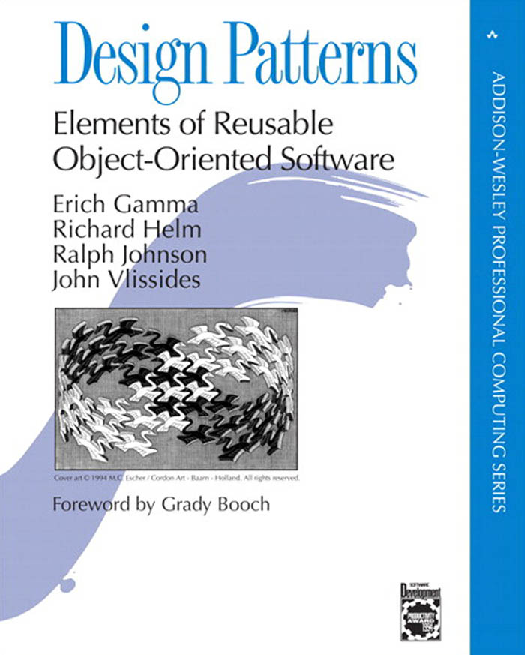
\includegraphics[width=\linewidth]{GoF}}		
	}
\end{frame}

\subsection{Template Method Pattern}
\begin{frame}{\insertsubsection}
	\leftorright{
		\mydefinition{Template Method \mysource{\gof}}{
			\begin{itemize}
				\item {\bf Intent:} \mycite{Define the overall structure of an algorithm, while allowing subclasses to refine, or redefine, certain steps.}
				\item {\bf Motivation:}  Avoid code replication by implementing the general workflow of an algorithm once, while allowing for necessary variations.
				\item {\bf Idea:} A template method defines the skeleton of an algorithm. Concrete methods override the hook methods.
			\end{itemize}
		}{}
	}{
		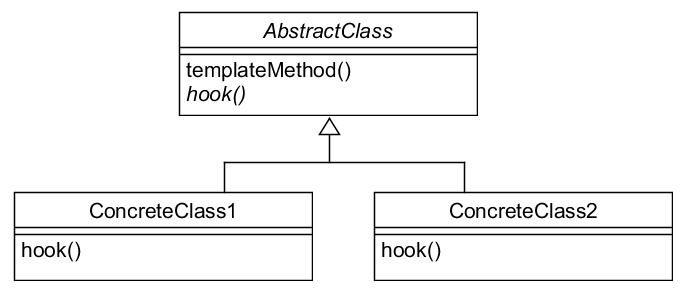
\includegraphics[width=\linewidth]{templatemethod}
	}
\end{frame}

\subsection{Abstract Factory Pattern}
\begin{frame}{\insertsubsection}
	\leftorright{
		\mydefinition{Abstract Factory \mysource{\gof}}{
			\begin{itemize}
				\item {\bf Intent:} \mycite{Provide an interface for creating families of related or dependent objects without specifying their concrete classes.}
				\item {\bf Motivation:} Avoid case distinctions when creating objects of certain kind, consistently create objects of a particular kind.
				\item {\bf Idea:} Create classes for the consistent creation of objects.
			\end{itemize}
		}{}
	}{
		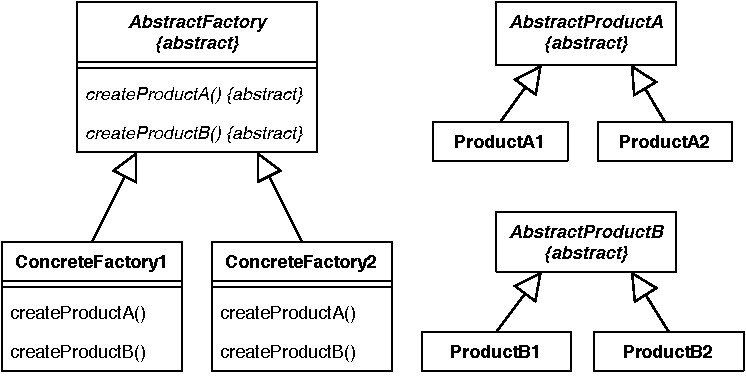
\includegraphics[width=\linewidth]{abstractfactory}
	}
\end{frame}

\subsection{Decorator Pattern}
\begin{frame}{\insertsubsection}
	\leftorright{
		\mydefinition{Decorator \mysource{\gof}}{
			\begin{itemize}
				\item {\bf Intent:} \mycite{Attach additional responsibilities to an object dynamically. Decorators provide a flexible alternative to subclassing for extending functionality.}
				\item {\bf Motivation:} Avoid explosion of static classes when combining all additional behaviors with all applicable classes.
				\item {\bf Idea:} Create decorators and components with the same interface, whereas decorators forward behavior whenever feasible.
			\end{itemize}
		}
	}{
		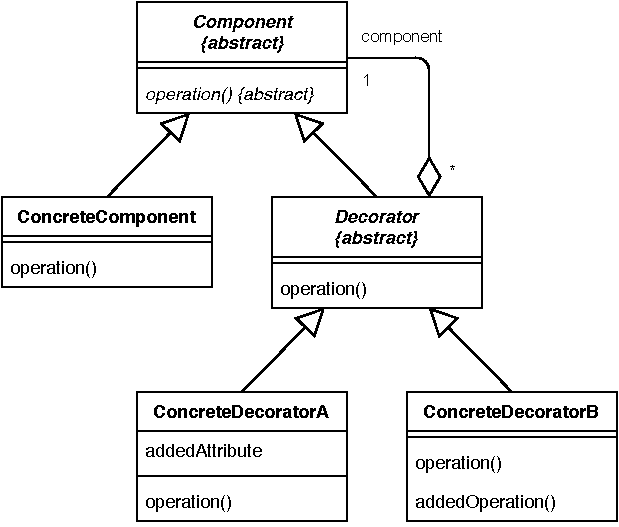
\includegraphics[width=\linewidth]{decorator}
	}
\end{frame}

\subsection{Object-Oriented Design of our Graph Library}
\begin{frame}{\insertsubsection}
	\leftorright{
		\begin{center}
			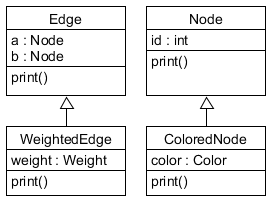
\includegraphics[width=0.7\linewidth]{graphlib-oo-node-edge.png}
		\end{center}		
	}{
		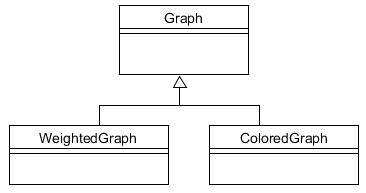
\includegraphics[width=\linewidth]{graphlib-oo-graph.png}	
	}
\end{frame}

\begin{frame}[fragile]{Instantiation through Template Method Pattern}
		\begin{columns}
			\column{.45\textwidth}
\begin{tiny}
\begin{lstlisting}
public class Graph {
	...
	Edge add(Node n, Node m) {
		Edge e = createEdge();
		nv.add(n); nv.add(m); ev.add(e);
		return e;
	}
	
	// hook method (with default implementation)
	Edge createEdge(Node n, Node m) {
		return new Edge(n, m);
	}
	...
}
\end{lstlisting}
\begin{lstlisting}
@public class WeightedGraph extends Graph {
	...
	// override hook method
	Edge createEdge(Node n, Node m) {
		Edge e = new WeightedEdge(n, m);
		e.weight = new Weight();
		return e;
	}
	...
}@
\end{lstlisting}
\end{tiny}	
			\column{.45\textwidth}
				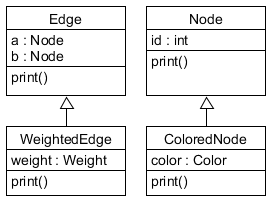
\includegraphics[width=0.75\linewidth]{graphlib-oo-node-edge}	
		\end{columns}
\end{frame}

\begin{frame}[fragile]{Instantiation through Abstract Factory Pattern}
		\begin{columns}
			\column{.45\textwidth}
\begin{tiny}
\begin{lstlisting}
public class Graph implements IGraph {
	EdgeFactory ef;
	...
	public Graph(EdgeFactory _ef) {
		ef = _ef;
	}
	
	public Edge add(Node n, Node m) {
		Edge e = ef.createEdge(n, m);
		nodes.add(n); nodes.add(m); edges.add(e);
		return e;
	}
	...
}
\end{lstlisting}
\begin{lstlisting}
public class EdgeFactory {
	Edge createEdge(Node a, Node b) {
		return new Edge(a, b);
	}
}
\end{lstlisting}
\begin{lstlisting}
@public class WeightedEdgeFactory extends EdgeFactory {
	Edge createEdge(Node a, Node b) {
		return new WeightedEdge(a, b);
	}
}@
\end{lstlisting}
\end{tiny}	
			\column{.45\textwidth}
				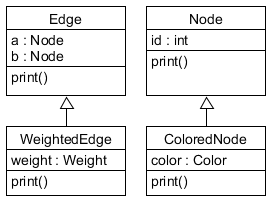
\includegraphics[width=0.75\linewidth]{graphlib-oo-node-edge}	
		\end{columns}
\end{frame}

\subsection{Feature Combinations}
\begin{frame}{Feature Combinations?}
	\leftorright{
		\begin{center}
			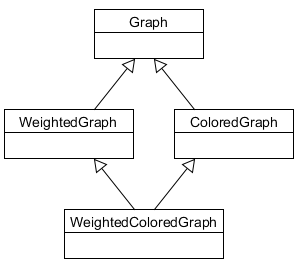
\includegraphics[width=\linewidth]{graphlib-oo-diamond}
		\end{center}		
	}{
	}
\end{frame}

\begin{frame}{Diamond Problem}
	\leftorright{
		\mynote{Multiple Inheritance}{
			\begin{itemize}
				\item Remember that most object-oriented programming languages do not support multiple inheritance (or only provide workarounds).
			\end{itemize}
		}
	}{
		\begin{center}
			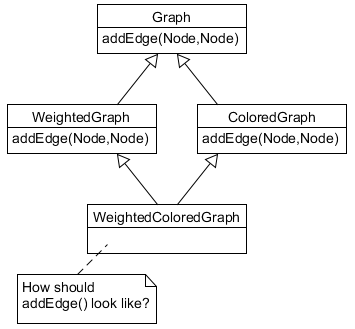
\includegraphics[width=\linewidth]{graphlib-oo-diamond-commented}
		\end{center}		
	}
\end{frame}

\begin{frame}{Static Modeling of Feature Combinations}
	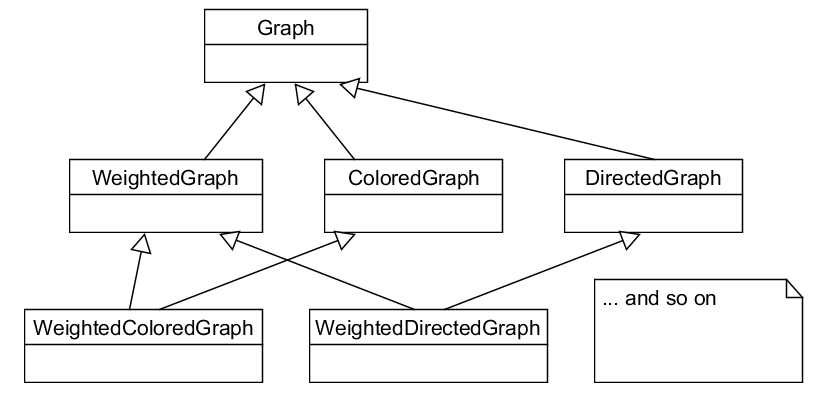
\includegraphics[width=0.7\linewidth]{graphlib-oo-combinatorial}
	\mynote{}{
		Even if multiple inheritance is supported, statically combining features through inheritance is tedious (or infeasible).
	}
\end{frame}

\begin{frame}[fragile]{Decorator Pattern as a Solution?}
		\begin{columns}
			\column{.45\textwidth}
\begin{tiny}
\begin{lstlisting}
public abstract class GraphDecorator implements IGraph {
	protected IGraph graph;
	
	public GraphDecorator(IGraph _graph) { 
		graph = _graph; 
	}
}
\end{lstlisting}
\begin{lstlisting}
@public class WeightedGraph extends GraphDecorator {
	public WeightedGraph(IGraph _graph) {
		super(_graph);
	}
	public Edge add(Node n, Node m) {
		WeightedEdge e = (WeightedEdge) graph.add(n, m);
		e.weight = new Weight();
		return e;
	}
	...
}@
\end{lstlisting}
\end{tiny}	
			\column{.45\textwidth}
				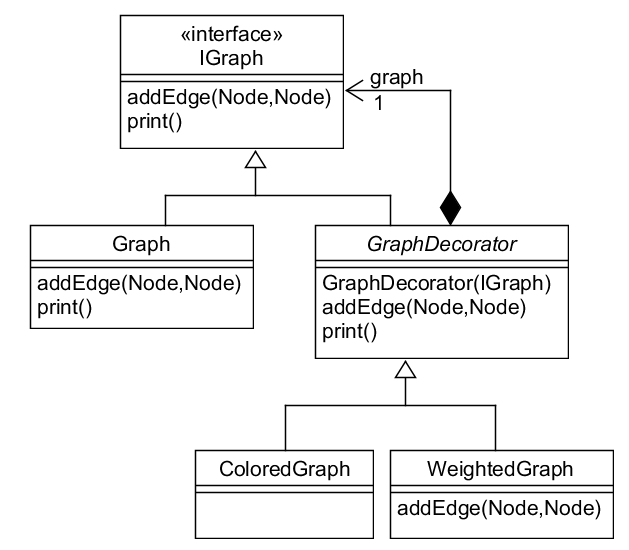
\includegraphics[width=\linewidth]{graphlib-oo-decorator}	
		\end{columns}
Usage Example: 
\begin{tiny}
\begin{lstlisting}
IGraph g = new WeightedGraph(new ColoredGraph(new Graph(new WeightedEdgeFactory())));
\end{lstlisting}
\end{tiny}	
\end{frame}

\begin{frame}{Delegation instead of Inheritance}
	\leftorright{
		\mynote{Discussion}{
			Extensions (i.e., features) can be combined dynamically, but \ldots
			\begin{itemize}
				\item \ldots must be independent of each other,
				\item \ldots cannot add public methods,
				\item \ldots plenty of indirections,
				\item \ldots several physical objects are forming a conceptual one.
			\end{itemize}
		}
	}{
		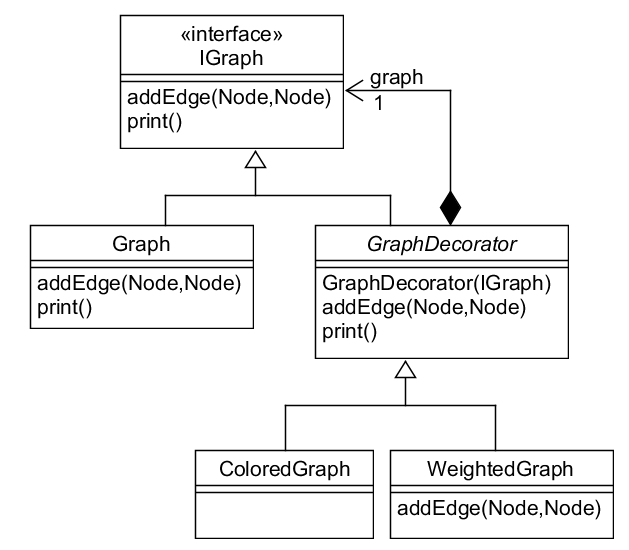
\includegraphics[width=\linewidth]{graphlib-oo-decorator}
	}
\end{frame}

\lessonslearned{
	\item Variability through object-orientation and design patterns
	\item Extension through delegation vs. inheritance  
	\item Limitations and drawbacks w.r.t. feature combinations
}{
	\item B. Meyer, Object-Oriented Software Construction, Prentice Hall, 1997. Chapters 3, 4
	\item E. Gamma, R. Helm, R. Johnson, and J. Vlissides. Design Patterns: Elements of Reusable Object-Oriented Software. Addison-Wesley, 1995.
}{
	\item What characterizes a modular software design and why can it support variability?
	\item In which sense are object-oriented solutions more modular than feature toggles?
	\item Do you know of other design patterns supporting variability?
}

\sectionend

\mode<beamer>{
	\begin{frame}{\inserttitle}
		\lectureseriesoverview
	\end{frame}

	\contentoverview
}


\end{document}
